\section{Theory}
\subsection{Background knowledge}
The paper proposes a new method for the task of image generation, which trains GANs using the quantum computer. GANs consist of two neural networks, a generator, and a discriminator. The job of the generator is to create synthetic data that is as close as possible to the real data, such as a text word or an image, whereas the discriminator tries to distinguish between the real data and generator-generated synthetic data. 

\subsection{Convergence}
The training process can be viewed as a zero-sum game, where the generator tries to minimize the value of the objective and the discriminator tries to maximize it. 

A GAN has \emph{converged} when the generator can no longer improve, or the discriminator can no longer distinguish between real and synthetic data. At this point, both two players have optimal strategies, and the generator has a 50\% chance of correctly distinguishing a generated image from a real one. 

\subsection{Training}

If the training converges, the objectives for the generator and discriminator should find the parameters $\theta$ for the generator and $\gamma$ for the discriminator that satisfy:

\[\min\limits_{\theta} \max\limits_{\gamma} \mathcal{L}\{D_{\gamma}{[G_{\theta}(z)], D_{\gamma}(x)}\} := \mathbb{E}_{x \sim P_{data}(x)}[\log D_{\gamma}(x)] + \mathbb{E}_{z \sim P(z)}(\log\{1 - D_{\gamma}[G_{\theta}(z)]\})\]

Where $D_{\gamma}(x)$ is the discriminator's estimate of the probability that training example $x$ is real, $\mathbb{E}_{x \sim P_{data}(x)}$ is the expected value over all training examples.
$G_{\theta}(z)$ is the generator's output when given noise $z$, $D_{\gamma}[G_{\theta}(z)]$ is the discriminator's estimate of the probability that a fake instance is real, and $\mathbb{E}_{z \sim P(z)}$ is the expected value over all random inputs to the generator. 

Specifically, for the discriminator, the loss is computed as the sum of the binary cross-entropy between the true labels (1 for real data and 0 for fake data) and the predicted probabilities. In other words, the discriminator aims to minimize the loss when correctly classifying real and fake examples. The lower the loss of the discriminator, the more effective the discriminator is in distinguishing between real and fake data.
For the generator, the loss is computed as the binary cross-entropy between the true labels and the discriminator's prediction of the generated data. The generator aims to maximize this loss because it means that the discriminator is classifying the synthetic data as real. In other words, the generator aims to produce synthetic data that minimize the discriminator's ability to distinguish between real and fake examples.

\subsection{Gradients}

We compute gradients for the discriminator's parameters in two configurations.  In Figure \ref{fig:discrim_fake}, the loss is minimized when discriminator identifies the generator's image as fake, while in Figure \ref{fig:discrim_real} it is minimized when it guessed that the training example is real.

\begin{figure}[H]
    \centering
    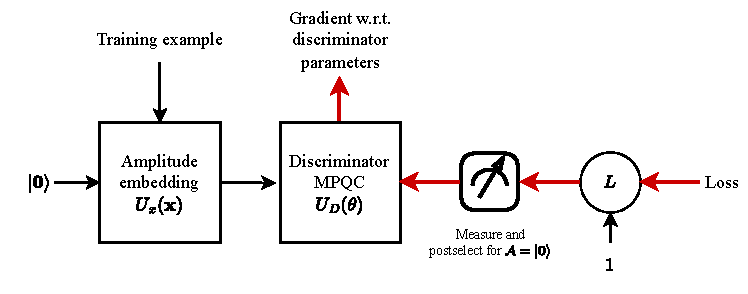
\includegraphics[width=0.7\textwidth]{figures/discrim_real.pdf}
    \caption{Gradients computation for the real example w.r.t. discriminator parameters.}
    \label{fig:discrim_real}
\end{figure}

\begin{figure}[H]
    \centering
    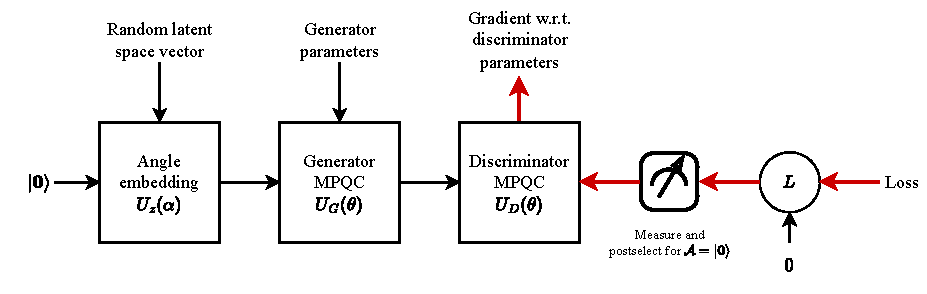
\includegraphics[width=0.8\textwidth]{figures/discrim_fake.pdf}
    \caption{Gradients computation for the fake example w.r.t. discriminator parameters.}
    \label{fig:discrim_fake}
\end{figure}

Gradients are computed for the generator in F
Figure \ref{fig:gen_fake}.  The same configuration is similar Figure \ref{fig:discrim_fake}, but the target label provided to the loss function is reversed.

\begin{figure}[H]
    \centering
    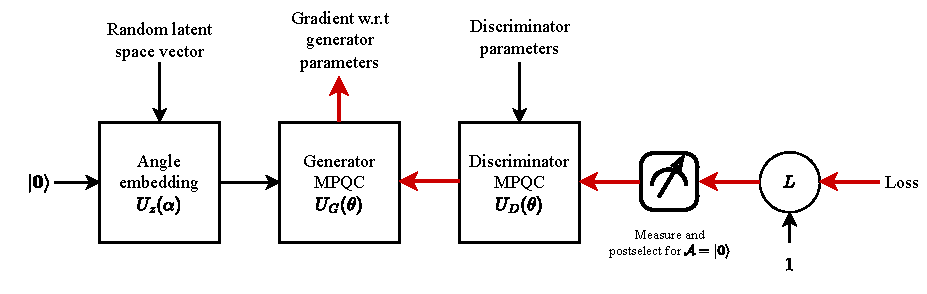
\includegraphics[width=0.8\textwidth]{figures/gen_fake.pdf}
    \caption{Gradients computation w.r.t. generator parameters.}
    \label{fig:gen_fake}
\end{figure}


\section{Quantum GANs}

Depending on the available quantum computing resources, the authors give two ways of 
getting some advantage when training a quantum circuit over a classical GAN:

\begin{itemize}
    \item When there are many more feature dimensions (for example, the $8\times 8$ MNIST digits used 
    as an example), we split up the feature vector and train many simple, independent quantum generators.
    Their output is stitched back together and fed to a single classical discriminator.  During training,
    gradients from the discriminator are back-propagated through the quantum GANs to obtain gradients with
    respect to their trainable parameters.  This is the ``patch'' strategy.  An implementation is available
    on the Pennylane blog\autocite{ellis2022quantum}, so we focus on implementing batch GANs only.

    \item When there are enough qubits to embed an entire training example into the amplitudes of the feature
    register, we train both a quantum generator and discriminator circuit.   With some additional qubits as an
    ``index register'', we can embed a superposition of training examples for an entire basis over the
    index register.  By training this circuit, we compute gradients for an entire batch training data
    with few additional gates.  This is called the ``batch strategy''.
\end{itemize}

\subsection{Multi-layer parameterized quantum circuits}

Both the generator and discriminator are multi-layer parameterized quantum circuits, which have
been shown to be more expressive than neural networks on a parameter-to-parameter basis in many
situations\autocite{zhai2022quantum}.

An MPQC consists of several layers of a repeating pattern: trainable gates (generally rotations so
that parameter shift derivatives can be taken), followed by a series of controlled gates to entangle the
resulting state.  Huang et. al use a structure like the one shown in figure \ref{fig:mpqc}, but 
MPQCs are flexible with respect to what gates are used, and in what order the entanglers are applied.

\begin{figure}[H]
    \centering
\begin{quantikz}
\qw & \gate{RY(\theta_{11})} & \ctrl{1} & \qw      & \gate{RY(\theta_{21})} & \ctrl{1} & \qw      & \qw \\
\qw & \gate{RY(\theta_{12})} & \ctrl{}  & \ctrl{1} & \gate{RY(\theta_{22})} & \ctrl{}  & \ctrl{1} & \qw \\
\qw & \gate{RY(\theta_{13})} & \qw      & \ctrl{}  & \gate{RY(\theta_{23})} & \qw      & \ctrl{}  & \qw \\
\end{quantikz}
    \caption{A two-layer MQPC using $RY$ gates as trainanbles, and $CZ$ gates for entangles, like the ones described in the paper.}
    \label{fig:mpqc}
\end{figure}


\subsection{Post-selection}

It is well known that ordinary neural networks need nonlinearities to be universal function
approximators\autocite{cybenko1989approximation}.  MPQCs must also be able to learn 
nonlinearity if they are to be useful for image generation.  This is accomplished by applying
the MPQC to extra ancillary qubits and throwing away measurements where the ancillary subsystem
is not in some fixed state.  We choose $\ket{0}$ arbitrarily.

\subsection{Batch GANs}

Figure \ref{fig:batch_gan} shows a high-level view of the entire batch GAN circuit.

\begin{figure}[H]
    \centering
\begin{quantikz}
\lstick[wires=1]{index $\ket{0}$}          & \gate[wires=4]{U(\bm{\alpha_z})} & \qw &              \qw & \qw                         \\
\lstick[wires=1]{gen. ancillary $\ket{0}$} & &                                  \gate[wires=3][2cm]{U_G(\bm{\theta})} & \qw &        \qw \rstick{$\ket{0}$} \\
\lstick[wires=2]{features $\ket{0}$}       & &                                  &                                      \gate[wires=3][2cm]{U_D(\bm{\gamma})} & \qw \\
                                           & \qw                             &  &                                                                         \qw  & \meter{} \\
\lstick[wires=1]{dis. ancillary $\ket{0}$} & \qw                             & \qw &\qw  &\qw \rstick{$\ket{0}$} \\
\end{quantikz}
    \caption{Schematic for batch GAN in the configuration used for training on generated examples.}
    \label{fig:batch_gan}
\end{figure}

The first unitary gate, $U(\bm{\alpha_z})$, is an angle embedding from the random latent space
onto the feature register (as well as generator ancillary and index register).  $U_G(\bm{\theta})$ and
$U_D(\bm{\gamma})$ are the MPQCs for the generator and discriminator respectively.  When training, we make a measurement,
throw it away if the ancillary bits are not zero, and estimate the probability that a non-ancillary bit of the discriminator's
output (in the feature register) is one.  This is the discriminator's probability that the given example is real.

When training with real images, the generator circuit is missing.  Instead, where $\bm{x}_i$ are training examples for $i\in\{1,\dots,k\}$,
an amplitude embedding initializes the index register and feature registers with the state:

\[-2^k \sum_{1\leq i\leq k} \ket{i}\otimes \bm{x}_i\]

The discriminator output is read off as normal.


